\documentclass[11pt,a4paper]{article}
\usepackage[utf8]{inputenc}
\usepackage[romanian]{babel}
\usepackage[margin=2.5cm]{geometry}
\usepackage{graphicx}
\usepackage{float}
\usepackage{tabularx}
\usepackage{longtable}
\usepackage{array}
\usepackage{multirow}
\usepackage{booktabs}
\usepackage{colortbl}
\usepackage{xcolor}
\usepackage{fancyhdr}
\usepackage{hyperref}
\usepackage{enumitem}
\usepackage{titlesec}

% Colors
\definecolor{headerblue}{RGB}{41,128,185}
\definecolor{lightgray}{RGB}{240,240,240}

% Page style
\pagestyle{fancy}
\fancyhf{}
\fancyhead[L]{\small FinGuard AI - Business Foundation}
\fancyhead[R]{\small \thepage}
\renewcommand{\headrulewidth}{0.4pt}

% Section formatting
\titleformat{\section}{\Large\bfseries}{\thesection.}{1em}{}
\titleformat{\subsection}{\large\bfseries}{\thesubsection}{1em}{}
\titleformat{\subsubsection}{\normalsize\bfseries}{\thesubsubsection}{1em}{}

% Hyperlinks
\hypersetup{
    colorlinks=true,
    linkcolor=blue,
    filecolor=blue,
    urlcolor=blue,
    citecolor=blue,
}

\setlength{\parindent}{0pt}
\setlength{\parskip}{6pt}

\begin{document}

% Title page
\begin{titlepage}
    \centering
    \vspace*{1cm}

    {\Large\textbf{Universitatea din București}}\\[0.3cm]
    {\Large\textbf{Facultatea de Matematică și Informatică}}\\[0.3cm]
    {\Large\textbf{Management de Produs și Antreprenoriat}}\\[1.5cm]

    {\Huge\textbf{Business Foundation}}\\[2cm]

    
\includegraphics[width=0.5\textwidth]{./assets/logo/logo.png}\\[1cm]

    {\LARGE\textbf{FinGuard AI}}\\[0.5cm]
    {\large\textit{Platformă SaaS de management financiar cu AI\\pentru freelanceri români}}\\[3cm]

    \vfill

    \begin{minipage}[t]{0.45\textwidth}
        \begin{flushleft}
            \textbf{Profesor coordonator:}\\
            Alin Ștefănescu
        \end{flushleft}
    \end{minipage}
    \hfill
    \begin{minipage}[t]{0.45\textwidth}
        \begin{flushright}
            \textbf{Studenți:}\\
            Clem Daria, 506\\
            Liciu Ștefan, 506\\
            Maftei Valentin, 506\\
            Nițoi Antonio, 506\\
            Sabău Eduard, 506\\
            Sandu Eduard, 506
        \end{flushright}
    \end{minipage}

    \vspace{1cm}
    {\large București, 2026}

\end{titlepage}

% Table of contents
{\small\tableofcontents}
\newpage

% Content
\section{Motivație}

\subsection{De ce există FinGuard AI?}

\textbf{Context 2026:}

Freelancing-ul și economia de tip "gig" au crescut exponențial în România post-pandemie. Conform datelor recente, peste \textbf{450.000 de PFA-uri active} și aproximativ \textbf{120.000 SRL-uri micro} deținute de freelanceri lucrează pe cont propriu în România (martie 2026). Cu toate acestea, managementul financiar și fiscal rămâne o provocare majoră pentru majoritatea acestora.

\textbf{Problema fundamentală:}

Freelancerii și micii antreprenori din România petrec în medie 8-12 ore pe lună pentru:
\begin{itemize}[nosep]
    \item Organizarea facturilor și chitanțelor
    \item Calcularea taxelor și impozitelor (CAS, CASS, impozit venit)
    \item Identificarea deducerilor fiscale posibile
    \item Previzionarea obligațiilor fiscale trimestriale
\end{itemize}

Această sarcină administrativă \textbf{consumă timp} ce ar putea fi dedicat activității productive, \textbf{generează anxietate} în legătură cu conformitatea fiscală, \textbf{conduce la erori} care pot rezulta în penalități financiare și \textbf{reduce profitabilitatea} prin neoptimizarea deducerilor legale.

\textbf{Impactul financiar al problemei:}

Pentru un freelancer IT cu venit mediu de 3.500 EUR/lună (tarif orar \textasciitilde35 EUR/h):
\begin{itemize}[nosep]
    \item \textbf{10 ore/lună} pentru administrare financiară = \textbf{350 EUR/lună pierdut} (\textasciitilde4.200 EUR/an)
    \item Risc penalități fiscale (întârzieri, erori): \textbf{500-2.000 RON/incident}
    \item Deduceri fiscale neoptimizate: \textbf{10-20\% din taxe} (estimat 1.000-3.000 RON/an)
    \item Cost angajare contabil: \textbf{300-500 RON/lună} (\textasciitilde3.600-6.000 RON/an)
\end{itemize}

\textbf{Cost total al problemei: 5.000-10.000 RON/an} pentru un freelancer activ.

\textbf{Cazuri de utilizare:}

\textbf{Cazul 1 - IT Freelancer (PFA):} Andrei, dezvoltator React cu 15-20 clienți/an, facturează 4.000 EUR/lună. Petrecea 12h/lună cu facturi, calcule CAS/CASS, și declarații. Cu FinGuard AI: 10 minute/lună, economie 420 EUR/lună timp + 1.500 RON/an prin optimizare deduceri.

\textbf{Cazul 2 - Consultant Marketing (SRL micro):} Maria, consultant digital marketing, 8-10 proiecte/an, venit 5.000 RON/lună. Plătea contabil 400 RON/lună. Cu FinGuard AI: 99 RON/lună, economie 3.600 RON/an + transparență completă asupra finanțelor.

\textbf{Cazul 3 - Designer Grafic (PFA):} Alexandru, designer freelance, 20-30 clienți mici/an, venit fluctuant 2.500-4.000 RON/lună. Anxietate constantă despre conformitate fiscală. Cu FinGuard AI: alertare proactivă, liniște sufletească, zero erori în declarații.

\textbf{Soluția noastră:}

FinGuard AI automatizează complet acest proces folosind agenți AI specializați, transformând managementul financiar dintr-o corvoadă în \textbf{cost fix de 49-199 RON/lună} cu \textbf{ROI de 300-500\%} prin economii de timp și optimizare fiscală. Platforma elimină fricțiunile administrative și oferă liniște sufletească fiscală freelancerilor, permițându-le să se concentreze pe ceea ce fac cel mai bine.

\section{Rezumat}

\subsection{Ce este FinGuard AI?}

\textbf{FinGuard AI} este o platformă SaaS (Software-as-a-Service) de management financiar bazată pe agenți AI, destinată freelancerilor și micilor antreprenori din România.

\subsection{Componente Principale}

\textbf{Agent 1: Expense Auditor}

Funcție: Scanare și clasificare automată a documentelor financiare folosind OCR + Vision AI (Claude 4.6 / GPT-4o).

Capabilități: încărcarea fotografiilor facturilor, extragerea automată a datelor (furnizor, sumă, dată, TVA, categorie), clasificarea automată pe categorii de deduceri fiscale conform Codului Fiscal RO, alertarea pentru documente incomplete, integrarea directă cu e-Factura ANAF, verificarea validității facturilor în SPV ANAF.

\textbf{Agent 2: Tax Strategy Advisor}

Funcție: Analiză cash-flow și optimizare fiscală folosind LLM (Claude/GPT) + Analytics + Tax Knowledge Base.

Capabilități: analiza fluxurilor financiare lunare și trimestriale, previzionarea taxelor datorate (CAS, CASS, impozit venit), sugestii de optimizare fiscală 100\% legale, alertarea pentru termenele-limită fiscale, simularea scenariilor financiare, recomandări pentru maximizarea deducerilor fiscale, rapoarte trimestriale și anuale gata de transmitere.

\subsection{User Flow Tipic}

Utilizatorul își creează cont și setează profilul fiscal (PFA, SRL micro, normă venit). Încarcă fotografii ale facturilor/chitanțelor sau activează integrarea automată cu e-Factura ANAF. Expense Auditor clasifică și extrage datele automat în $<$ 5 secunde. Tax Advisor analizează periodic și trimite rapoarte + recomandări. La finalul trimestrului, raport complet cu taxele datorate și optimizări.

\subsection{Beneficii Concrete pentru Utilizatori}

\textbf{Economii de timp măsurabile:}
\begin{itemize}[nosep]
    \item De la \textbf{8-12 ore/lună} la \textbf{10 minute/lună} (reducere 98\%)
    \item Clasificarea automată a facturilor în $<$5 secunde vs 5-10 minute manual
    \item Rapoarte trimestriale generate instant vs 2-3 ore compilare manuală
    \item Zero timp petrecut cu calcularea CAS/CASS/impozit (100\% automatizat)
\end{itemize}

\textbf{Economii financiare:}
\begin{itemize}[nosep]
    \item Optimizare deduceri fiscale: \textbf{500-2.000 RON/an economisiți}
    \item Evitare penalități (întârzieri, erori): \textbf{0 vs 500-2.000 RON/incident}
    \item Cost vs contabil: \textbf{49-199 RON/lună vs 300-500 RON/lună} (economie 50-70\%)
    \item ROI mediu estimat: \textbf{300-500\%} în primul an
\end{itemize}

\textbf{Liniște sufletească (beneficiu nemăsurabil):}
\begin{itemize}[nosep]
    \item Alertare proactivă pentru termenele-limită (zero întârzieri)
    \item Conformitate 100\% cu legislația fiscală RO (actualizată continuu)
    \item Recomandări de optimizare fiscală 100\% legale (fără risc)
    \item Transparență completă: vezi exact cât datorezi și de ce
\end{itemize}

\subsection{De ce FinGuard AI este diferit?}

\textbf{1. AI-first, nu automatizare tradițională:}

SmartBill/Oblio oferă automatizarea fluxurilor de lucru (șabloane facturi, sincronizare ANAF), dar \textbf{fără inteligență}. FinGuard AI \textbf{înțelege} contextul fiscal, \textbf{învață} din comportamentul tău, \textbf{recomandă} proactiv optimizări.

\textbf{Exemplu concret:} Upload factură transport Uber pentru meeting cu client. SmartBill: "Ai adăugat o cheltuială de 45 RON". FinGuard AI: "Cheltuială de transport 45 RON clasificată ca DEDUCTIBILĂ 100\% (deplasare business). Economie fiscală estimată: 7 RON (16\% impozit)."

\textbf{2. Specializare legislație RO (nu generic internațional):}

QuickBooks/FreshBooks/Wave sunt excelente global, dar \textbf{nu știu nimic despre legislația RO}. FinGuard AI este antrenat specific pe Codul Fiscal RO 2026, OUG 89/2025, cote CAS/CASS, SPV ANAF, e-Factura.

\textbf{3. Proactiv, nu reactiv:}

Competiția: "Ai depășit termenul-limită al declarației, plătește penalitate". FinGuard AI: "În 14 zile este termenul-limită pentru declarația CAS. Estimare sumă datorată: 1.240 RON. Recomandare: poți deduce încă 350 RON din cheltuieli de transport pentru acest trimestru."

\textbf{4. De ce acum este momentul potrivit (2026)?}

\begin{itemize}[nosep]
    \item \textbf{Maturizarea AI:} Claude 4.6/GPT-4o permit reasoning complex legislație fiscală
    \item \textbf{Digitalizare ANAF obligatorie:} 100\% până 2028, freelancerii să aibă soluții digitale
    \item \textbf{Gap competitiv masiv:} Zero AI players în RO (SmartBill/Oblio = tech 2015)
    \item \textbf{First-mover advantage:} 18-24 luni până competiția reacționează
    \item \textbf{Post-pandemie boom:} 570k TAM, creștere 7-10\%/an, maturizare freelancing RO
\end{itemize}

\section{Detalii privind soluția propusă}

\subsection{Analiza SWOT}

\begin{figure}[H]
\centering
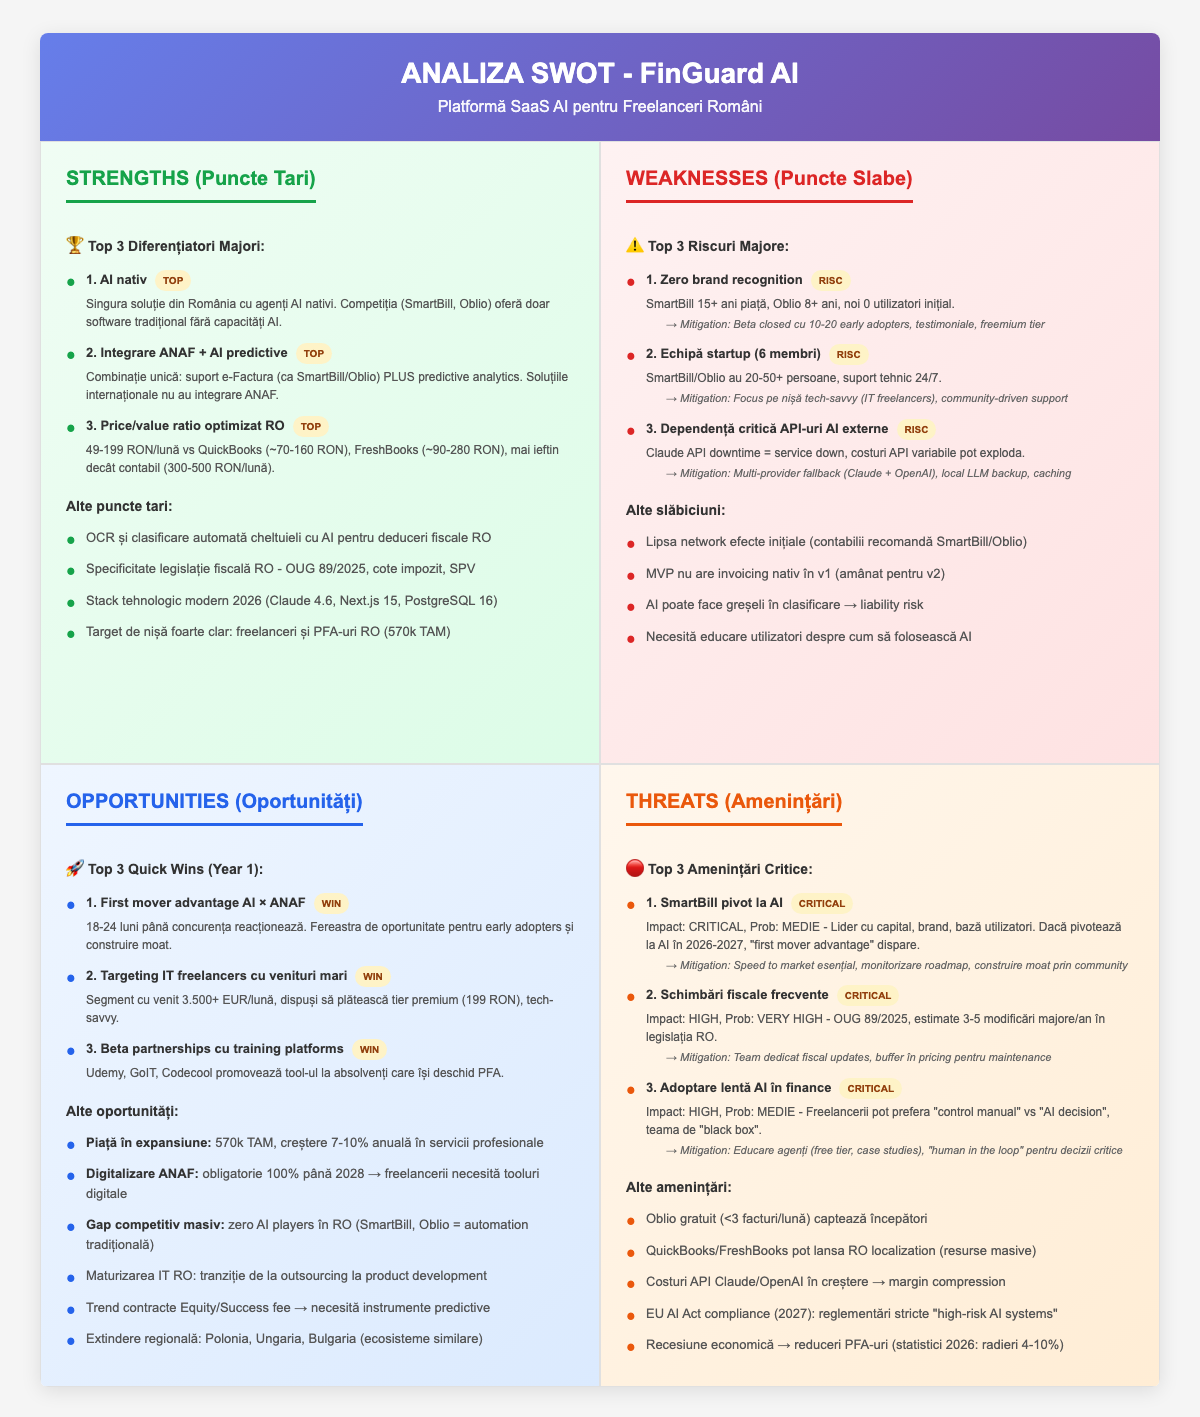
\includegraphics[width=\textwidth]{./assets/diagrams/swot-analysis.png}
\caption{Analiza SWOT - FinGuard AI (Strengths, Weaknesses, Opportunities, Threats)}
\end{figure}

\textbf{Rezumat SWOT:}

\textbf{Strengths (Puncte Tari):} AI nativ (singura soluție RO cu agenți AI), Integrare ANAF + AI predictive, Price/value ratio optimizat (49-199 RON/lună), OCR și clasificare automată pentru deduceri fiscale RO, specificitate legislație RO, stack tehnologic modern 2026.

\textbf{Weaknesses (Puncte Slabe):} Zero brand recognition (SmartBill 15+ ani, Oblio 8+ ani vs noi 0), echipă startup (6 membri vs 20-50+), dependență API-uri AI externe. Mitigation: Beta cu early adopters, focus nișă tech-savvy, multi-provider fallback.

\textbf{Opportunities (Oportunități):} First mover advantage AI × ANAF (18-24 luni), targeting IT freelancers venituri mari (3.500+ EUR/lună), beta partnerships cu training platforms, piață în expansiune (570k TAM, +7-10\%/an), digitalizare ANAF 100\% până 2028, gap competitiv masiv (zero AI players RO).

\textbf{Threats (Amenințări):} SmartBill pivot la AI (CRITICAL), schimbări fiscale frecvente (3-5/an), adoptare lentă AI în finance. Mitigation: Speed to market, team dedicat fiscal updates, educare users + human-in-loop.

\subsection{Market Analysis}

\subsubsection{Dimensiunea Pieței}

\textbf{TAM} (Total Addressable Market): \textasciitilde570.000 potențiali utilizatori (450k PFA + 120k SRL micro).

\textbf{SAM} (Serviceable Addressable Market): \textasciitilde300.000 utilizatori cu venituri $>$3.000 RON/lună (IT, Marketing, Consultanță, Design, Legal).

\textbf{SOM} (Serviceable Obtainable Market) An 1: 1.500-3.000 utilizatori plătitori (0.5-1\% SAM).

\subsubsection{Statistici Piață Freelancing România}

\textbf{Venituri medii:} Media generală 4.800-6.200 RON net/lună, IT Seniori 3.500-4.500 EUR net/lună, Remote Global Workers \textasciitilde3.500 USD/lună.

\textbf{Domenii active:} IT \& Software Development, Marketing Digital \& Content AI, Consultanță \& Legal, Educație Online \& Coaching.

\textbf{Predicții creștere (2026-2028):} Digitalizare ANAF 100\% până 2028, creștere anuală 7-10\% servicii profesionale.

\subsubsection{Analiza Competitorilor}

\textbf{Competitori Locali:}

\textbf{SmartBill} - Liderul pieței RO. Pricing: 25-75+ RON/lună. Avantaje: conformitate 100\% legislație RO, suport excelent, ecosistem vast integrări. Dezavantaje: interfață aglomerată, fără capacități AI.

\textbf{Oblio} - Concurent agresiv. Pricing: \textasciitilde180-250 RON/an (\textasciitilde15-21 RON/lună), gratuit $<$3 facturi/lună. Avantaje: simplitate radicală, preț competitiv. Dezavantaje: mai puține integrări, fără capacități AI.

\textbf{Competitori Internaționali:}

\textbf{QuickBooks Self-Employed} - Soluție globală Intuit. Pricing: \$15-35/lună (\textasciitilde70-160 RON). Avantaje: best mobile app, OCR basic. Dezavantaje: fără integrare ANAF, calcul taxe irelevant pentru RO.

\textbf{FreshBooks} - Focusat pe "time sellers". Pricing: \$19-60+/lună (\textasciitilde90-280 RON). Avantaje: time-tracking nativ, prezentare frumoasă. Dezavantaje: pricing crește rapid, fără integrare ANAF.

\textbf{Wave Accounting} - Free tier best-in-class. Pricing: 0 USD (core features). Avantaje: singura soluție profesională gratuită. Dezavantaje: fără suport bănci RO, fără e-Factura.

\begin{table}[H]
\centering
\small
\begin{tabular}{|l|c|c|c|c|c|c|}
\hline
\rowcolor{lightgray}
\textbf{Funcționalitate} & \textbf{FinGuard} & \textbf{SmartBill} & \textbf{Oblio} & \textbf{QBooks} & \textbf{Fresh} & \textbf{Wave} \\
\hline
AI Expense Classification & DA & NU & NU & NU & NU & NU \\
\hline
AI Tax Advisor & DA & NU & NU & NU & NU & NU \\
\hline
OCR Facturi & DA & NU & NU & DA & NU & DA \\
\hline
Integrare ANAF & DA & DA & DA & NU & NU & NU \\
\hline
Legislație RO & DA & DA & DA & NU & PARTIAL & NU \\
\hline
Preț/lună (RON) & \textbf{49-199} & 25-75 & 15-21 & 70-160 & 90-280 & \textbf{0} \\
\hline
\end{tabular}
\caption{Matrice Funcționalități Comparative}
\end{table}

\subsubsection{Diferențiatori Cheie}

\textbf{1. Abordare AI-first nativă} - Singura soluție RO cu agenți AI nativi.

\textbf{2. Integrare ANAF + AI predictiv} - Suport e-Factura + analiză predictivă.

\textbf{3. Specificitate legislație RO} - Deep knowledge Cod Fiscal RO (OUG 89/2025).

\textbf{4. Preț competitiv optimizat} - Sub QuickBooks/FreshBooks, comparabil SmartBill/Oblio.

\textbf{5. Automatizare end-to-end} - De la factură la raport ANAF, zero manual work.

\subsection{Tehnologii Folosite}

\textbf{Backend/AI Engine:} NestJS 11 pentru API, Google Cloud Firestore pentru persistența datelor si procesarea documentelor financiare. Anthropic Claude 4.6 API (Sonnet/Opus/Haiku), Gemini 3 Flash Preview, OpenAI GPT-4o (fallback) raman componentele principale ale stratului AI si de procesare asincronă.

\textbf{Frontend:} React 19/Vite, TypeScript 6, Tailwind CSS 4, shadcn/ui, Firebase hosting.

\textbf{DevOps:} Railway (MVP backend), GitHub Actions (CI/CD), Docker, Sentry (error tracking), PostHog (analytics), Better Stack (logging), Cloudflare R2 pentru storage.

\textbf{Security:} Firebase Authentication (OAuth 2.0, Google Sign-In), GDPR Compliance (data residency EU), encryption (TLS 1.3 transit, AES-256 at rest).

\textbf{Integrări:} ANAF e-Factura API (RO238), ANAF SPV API, Stripe + Netopia Payments, OpenBanking/PSD2 (post-v2).

\textbf{Costuri estimate lunare MVP (50-200 users):} Infrastructure + APIs 2.300-7.000 RON, Monitoring \& Security 180-425 RON, Development Tools 450-750 RON. \textbf{Total: 2.300-4.000 RON/lună} (growth: 4.500-7.000 RON).

\subsection{Riscuri Posibile}

\begin{table}[H]
\centering
\small
\begin{tabularx}{\textwidth}{|l|l|c|c|X|}
\hline
\rowcolor{lightgray}
\textbf{Risc} & \textbf{Tip} & \textbf{Impact} & \textbf{Prob.} & \textbf{Mitigation} \\
\hline
Modificări legislative & Business & HIGH & HIGH & Team monitorizare ANAF, update $<$48h \\
\hline
Costuri API AI & Financiar & MED & MED & Deploy LLM local, caching, multi-provider \\
\hline
Adoptare lentă & Business & HIGH & MED & Free tier 30 zile, case studies, human-in-loop \\
\hline
SmartBill/Oblio AI & Business & HIGH & MED & Speed to market, focus nișă, community \\
\hline
Probleme ANAF & Tehnic & MED & MED & Redundancy, cache, manual fallback \\
\hline
Erori clasificare AI & Legal & MED & MED & Disclaimer ToS, human review, audit trail \\
\hline
Concurență QBooks RO & Business & MED & LOW & Focus nișă RO, inovație continuă \\
\hline
Vulnerabilități security & Tehnic & HIGH & MED & Security audits, bug bounty, pentesting \\
\hline
Dependență vendor AI & Tehnic & MED & MED & Multi-provider, local LLM backup \\
\hline
Reglementări AI (EU) & Legal & MED & LOW & Transparency by design, human-in-loop \\
\hline
\end{tabularx}
\caption{Top 10 Riscuri Identificate}
\end{table}

\section{Planificare}

\subsection{Echipa}

\textbf{Număr membri:} 6 fondatori (doar equity în faza bootstrapped)

\textbf{Background echipă:} Toți membrii sunt studenți/absolvenți Facultatea de Matematică și Informatică, Universitatea București, cu experiență în dezvoltare software și proiecte IT. Echipa combină expertiză tehnică solidă cu cunoștințe de bază în management de produs și growth, acumulate prin proiecte academice și internship-uri.

\begin{table}[H]
\centering
\small
\begin{tabularx}{\textwidth}{|l|l|X|}
\hline
\rowcolor{lightgray}
\textbf{Nume} & \textbf{Rol} & \textbf{Responsabilități} \\
\hline
Sabău Eduard & Tech Lead \& Backend & Arhitectură sistem, AI/ML integration, ANAF APIs, coordonare echipă \\
\hline
Maftei Valentin & Backend Engineer & Database design, API development, security, integrări banking \\
\hline
Liciu Ștefan & AI/ML Engineer & AI agents, prompt engineering, OCR, Qdrant vector DB \\
\hline
Sandu Eduard & Frontend Engineer & Web app UI/UX, React, state management, fluxuri principale web \\
\hline
Clem Daria & Product \& Strategy & Roadmap, cercetare utilizatori, prioritizare features, UX \\
\hline
Nițoi Antonio & Growth \& Community & Content tehnic (blog, docs), community building, developer relations \\
\hline
\end{tabularx}
\caption{Echipa FinGuard AI}
\end{table}

\textbf{Model de compensație:} Doar equity pentru primele 12-18 luni. Tranziția la salarii după break-even + 3-6 luni rezervă de cash (luna 12-15). Reduce rata de ardere a capitalului la \textasciitilde4.000-12.000 RON/lună vs \textasciitilde45.000+ cu salarii.

\subsection{Milestones}

\begin{table}[H]
\centering
\small
\begin{tabularx}{\textwidth}{|l|c|X|}
\hline
\rowcolor{lightgray}
\textbf{Jalon} & \textbf{Durată} & \textbf{Activități Cheie} \\
\hline
M0: Research \& Setup & 2 săpt & Analiză competiție, validare, setup infra, mockups \\
\hline
M1: MVP Backend & 4 săpt & Auth, User profiles, Document upload, ANAF integration \\
\hline
M2: AI Agents Core & 4 săpt & Expense Auditor (OCR), Tax Advisor \\
\hline
M3: MVP Frontend & 3 săpt & Dashboard, Upload interface, Reports \\
\hline
M4: Integration \& Testing & 2 săpt & E2E testing, Security audit, Performance \\
\hline
M5: Beta Launch & 2 săpt & Closed beta (10-20 users), Feedback, Bug fixes \\
\hline
M6: Public Launch v1.0 & 2 săpt & Marketing campaign, Public release, Support \\
\hline
\end{tabularx}
\caption{Cronologie Proiect: \textasciitilde19 săptămâni (Aprilie - August 2026)}
\end{table}

\subsection{Diagrama Gantt}

\begin{figure}[H]
\centering
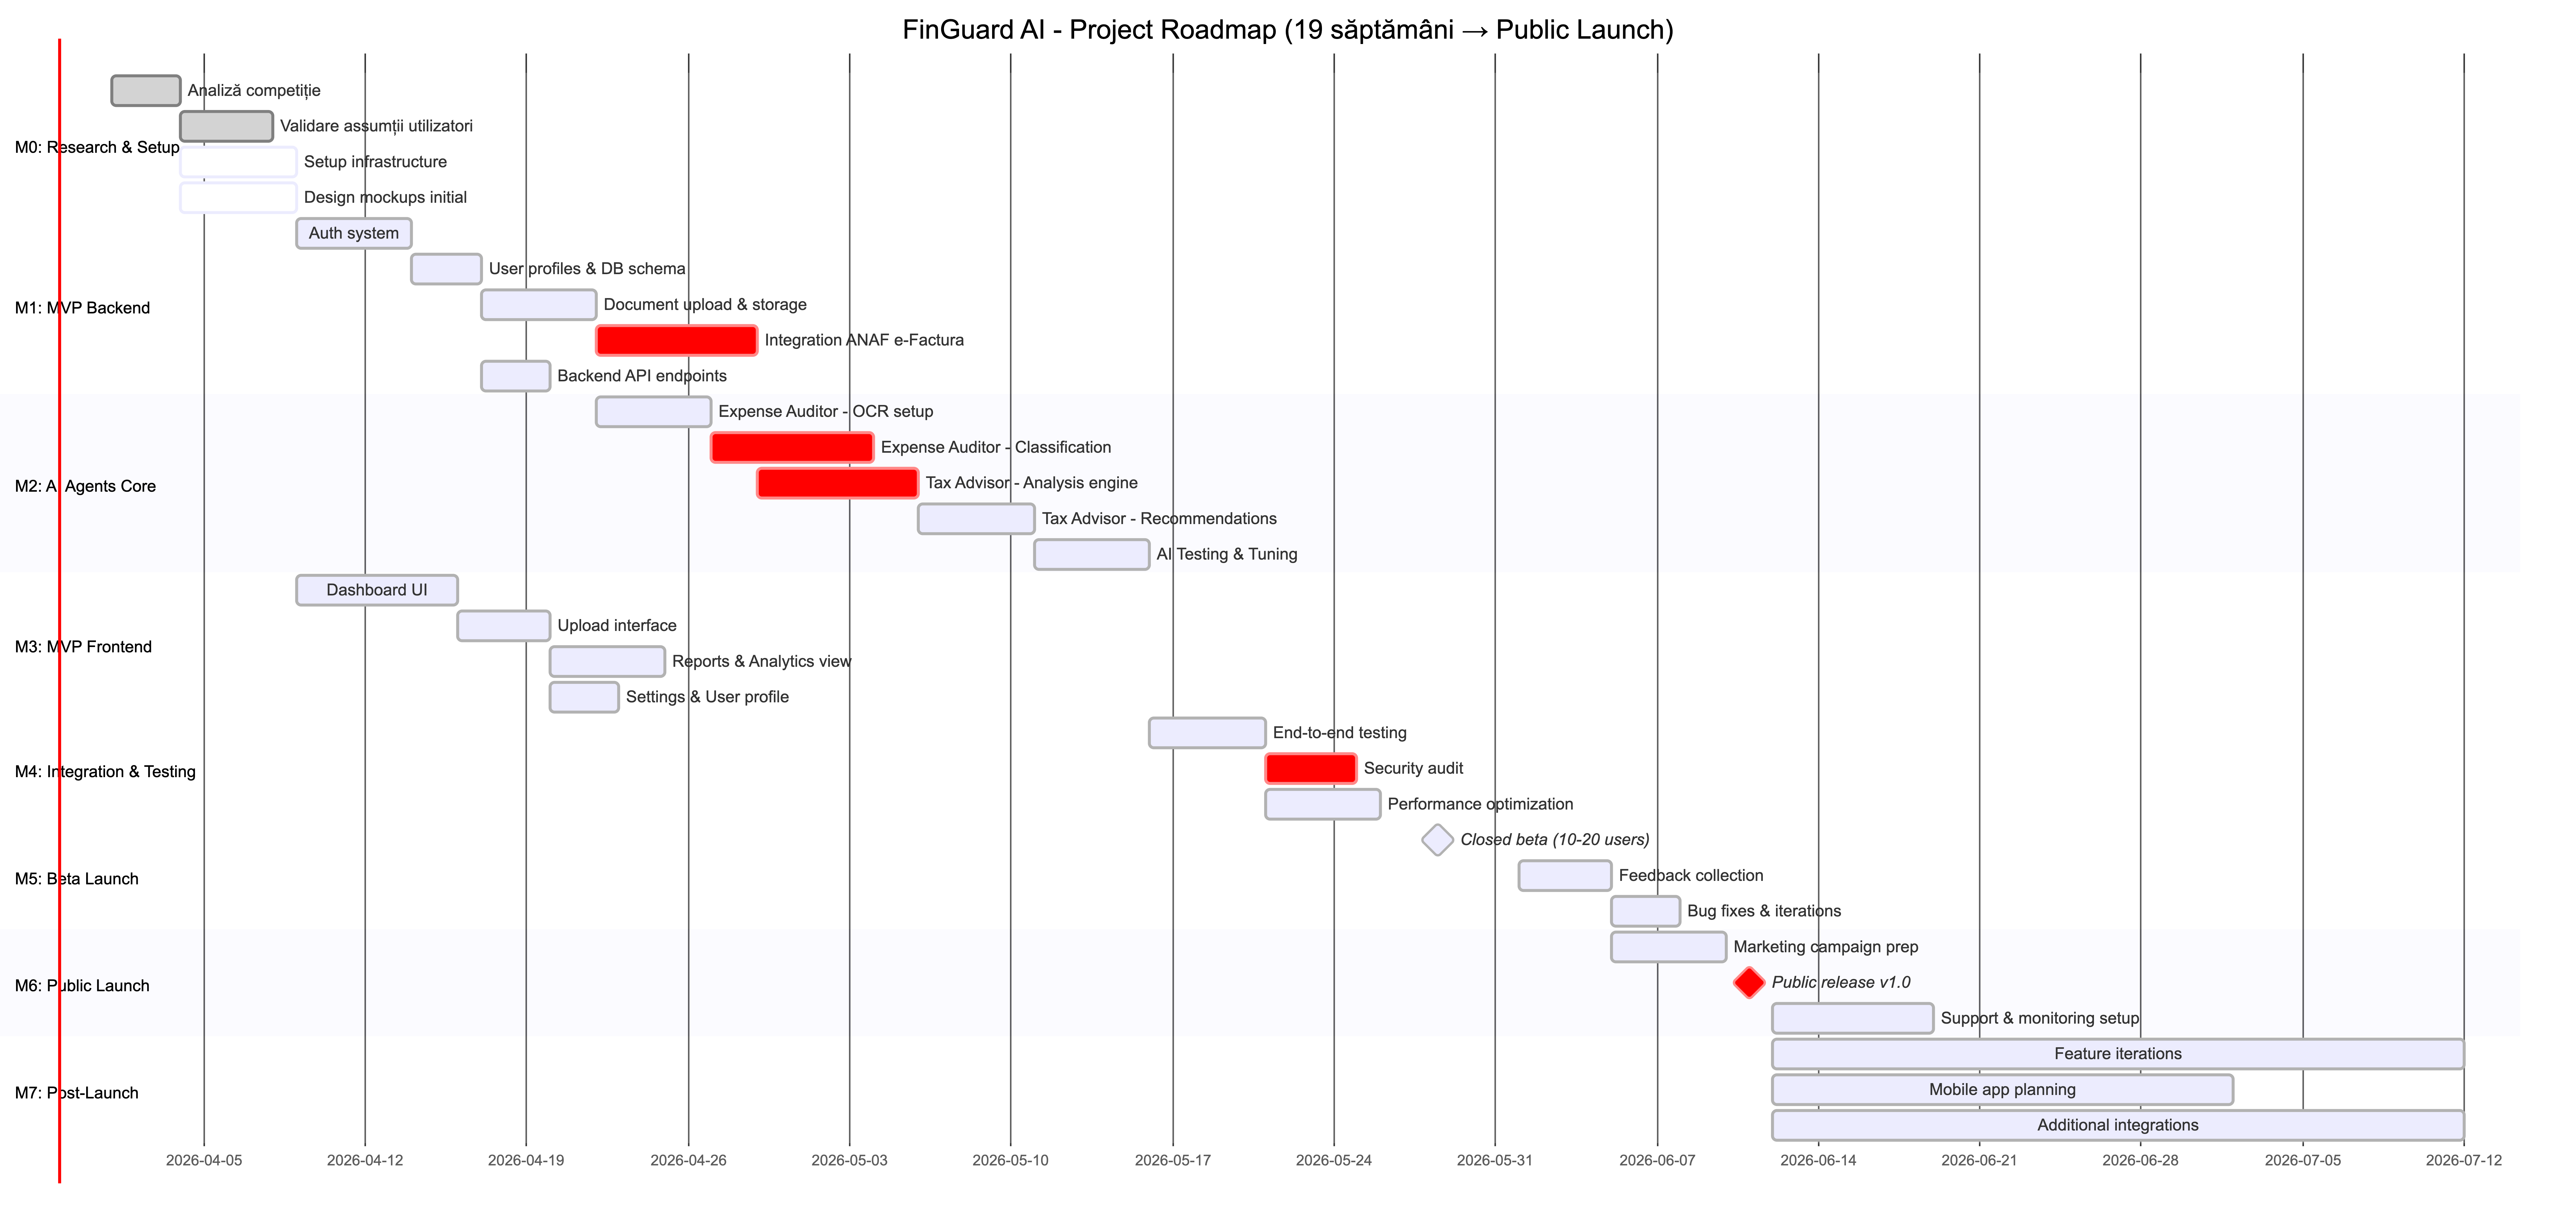
\includegraphics[width=0.95\textwidth]{./assets/diagrams/gantt.png}
\caption{Diagrama Gantt - FinGuard AI Project Roadmap (7 jaloane, descompunere task-uri, dependențe, traseu critic, paralelizare)}
\end{figure}

\section{Costuri}

\subsection{Categorii de Costuri}

\textbf{Costuri Inițiale} (one-time): Înființare SRL, design logo \& branding, legal setup (ToS, Privacy Policy), infrastructure setup.

\textbf{Costuri Recurente} (lunare): Salarii echipă (sau equity), servicii cloud, API-uri AI, tools \& licențe, marketing, juridic \& contabilitate.

\textbf{Costuri Variabile}: Proporționale cu utilizatori (API calls, storage, bandwidth).

\subsection{Estimări de Costuri}

\subsubsection{Costuri Inițiale}

\begin{table}[H]
\centering
\begin{tabular}{|l|r|}
\hline
\rowcolor{lightgray}
\textbf{Categorie} & \textbf{Cost (RON)} \\
\hline
Înființare SRL & 1.500 \\
Design branding & 2.000 \\
Legal setup & 3.000 \\
Website/landing & 3.000 \\
Infrastructure & 500 \\
\hline
\rowcolor{lightgray}
\textbf{TOTAL INIȚIAL} & \textbf{10.000} \\
\hline
\end{tabular}
\end{table}

\subsubsection{Costuri Lunare}

\textbf{Scenariul Bootstrapped (ALES):}

\begin{table}[H]
\centering
\begin{tabular}{|l|r|l|}
\hline
\rowcolor{lightgray}
\textbf{Categorie} & \textbf{Cost/lună (RON)} & \textbf{Notă} \\
\hline
Infrastructure + APIs & 2.300-7.000 & Managed Node hosting, Claude API, storage obiecte \\
Marketing \& Ads & 1.000-3.000 & Google Ads, SEO \\
Juridic \& Contabilitate & 500-1.000 & Lunar, contracte \\
Altele (buffer) & 500 & Unexpected \\
\textbf{Salarii} & \textbf{0} & \textbf{Founders pe EQUITY} \\
\hline
\rowcolor{lightgray}
\textbf{TOTAL LUNAR} & \textbf{4.000-12.000} & \textbf{Medie \textasciitilde10.000/lună} \\
\hline
\end{tabular}
\end{table}

\textbf{Scenariul cu Finanțare} (comparație):

\begin{table}[H]
\centering
\begin{tabular}{|l|r|}
\hline
\rowcolor{lightgray}
\textbf{Categorie} & \textbf{Cost/lună (RON)} \\
\hline
Infrastructure + APIs & 2.300-7.000 \\
Salarii 6 membri & 37.000-40.000 \\
Marketing & 2.000-5.000 \\
Juridic & 500-1.000 \\
\hline
\rowcolor{lightgray}
\textbf{TOTAL LUNAR} & \textbf{45.000-55.000} \\
\hline
\end{tabular}
\end{table}

\subsubsection{Costuri Anuale (Anul 1)}

\textbf{Scenariul Bootstrapped (ALES):}
\begin{itemize}[nosep]
    \item Costuri inițiale: 10.000 RON
    \item Costuri lunare: 10.000 × 12 = 120.000 RON
    \item \textbf{TOTAL AN 1: 130.000 RON}
\end{itemize}

\textbf{Scenariul cu Finanțare} (comparație): TOTAL AN 1: \textasciitilde550.000 RON

\textbf{Optimizări cost-eficiență:} Railway vs AWS (economie \textasciitilde\$300-500/lună), Cloudflare R2 vs S3 (economie \textasciitilde\$100-200/lună), niveluri gratuite (Vercel, Clerk, PostHog). \textbf{Total economii: \textasciitilde60\% reducere} vs AWS + servicii gestionate tradiționale.

\subsection{Model de Business}

\subsubsection{Pricing Tiers}

\begin{table}[H]
\centering
\begin{tabular}{|l|r|l|}
\hline
\rowcolor{lightgray}
\textbf{Plan} & \textbf{Preț/lună (RON)} & \textbf{Target} \\
\hline
Free Tier & 0 & Trial (10 docs/lună, 30 zile) \\
Starter & 49 & Freelanceri începători \\
Professional & 99 & Freelanceri activi \\
Business & 199 & SRL micro, agenții \\
\hline
\end{tabular}
\end{table}

\subsubsection{Proiecții Venituri An 1}

\begin{table}[H]
\centering
\small
\begin{tabular}{|c|r|r|r|r|r|}
\hline
\rowcolor{lightgray}
\textbf{Lună} & \textbf{Free} & \textbf{Starter} & \textbf{Pro} & \textbf{Business} & \textbf{Venit (RON)} \\
\hline
1 & 20 & 0 & 0 & 0 & 0 \\
2 & 35 & 5 & 0 & 0 & 245 \\
3 & 50 & 10 & 2 & 0 & 688 \\
4 & 70 & 20 & 5 & 1 & 1.678 \\
5 & 95 & 35 & 10 & 2 & 3.103 \\
6 & 120 & 55 & 18 & 3 & 5.179 \\
7 & 150 & 80 & 30 & 5 & 8.915 \\
8 & 180 & 110 & 45 & 8 & 13.447 \\
9 & 210 & 145 & 65 & 12 & 19.040 \\
10 & 250 & 185 & 90 & 18 & 26.475 \\
11 & 300 & 230 & 120 & 25 & 35.250 \\
12 & 350 & 280 & 155 & 35 & 45.835 \\
\hline
\rowcolor{lightgray}
\textbf{TOTAL} & - & - & - & - & \textbf{159.855} \\
\hline
\end{tabular}
\caption{Proiecții de Venituri Conservatoare - Anul 1}
\end{table}

\subsection{Analiza Cost-Beneficiu}

\textbf{Scenariul Bootstrapped (ALES):}

\begin{itemize}[nosep]
    \item \textbf{Costuri An 1:} 130.000 RON
    \item \textbf{Venituri An 1:} 159.855 RON (conservator)
    \item \textbf{Profit Net An 1:} +29.855 RON (profitabil în primul an!)
\end{itemize}

\textbf{ROI (Return on Investment):}
\[ ROI = \frac{159.855 - 130.000}{130.000} \times 100\% \approx 23\% \]

\textbf{Break-even:} Luna 9-10 (venituri cumulate depășesc costuri cumulate)

\textbf{Metrici Cheie:}
\begin{itemize}[nosep]
    \item \textbf{LTV} (Valoare pe durata de viață): 1.200-2.400 RON (12-24 luni retenție)
    \item \textbf{CAC} (Cost de achiziție client): $<$300 RON/client
    \item \textbf{Raport LTV:CAC:} 4-8:1 (sănătos: $>$3:1)
    \item \textbf{Marjă brută:} \textasciitilde60-70\%
\end{itemize}

\section{Lean Canvas}

\begin{figure}[H]
\centering
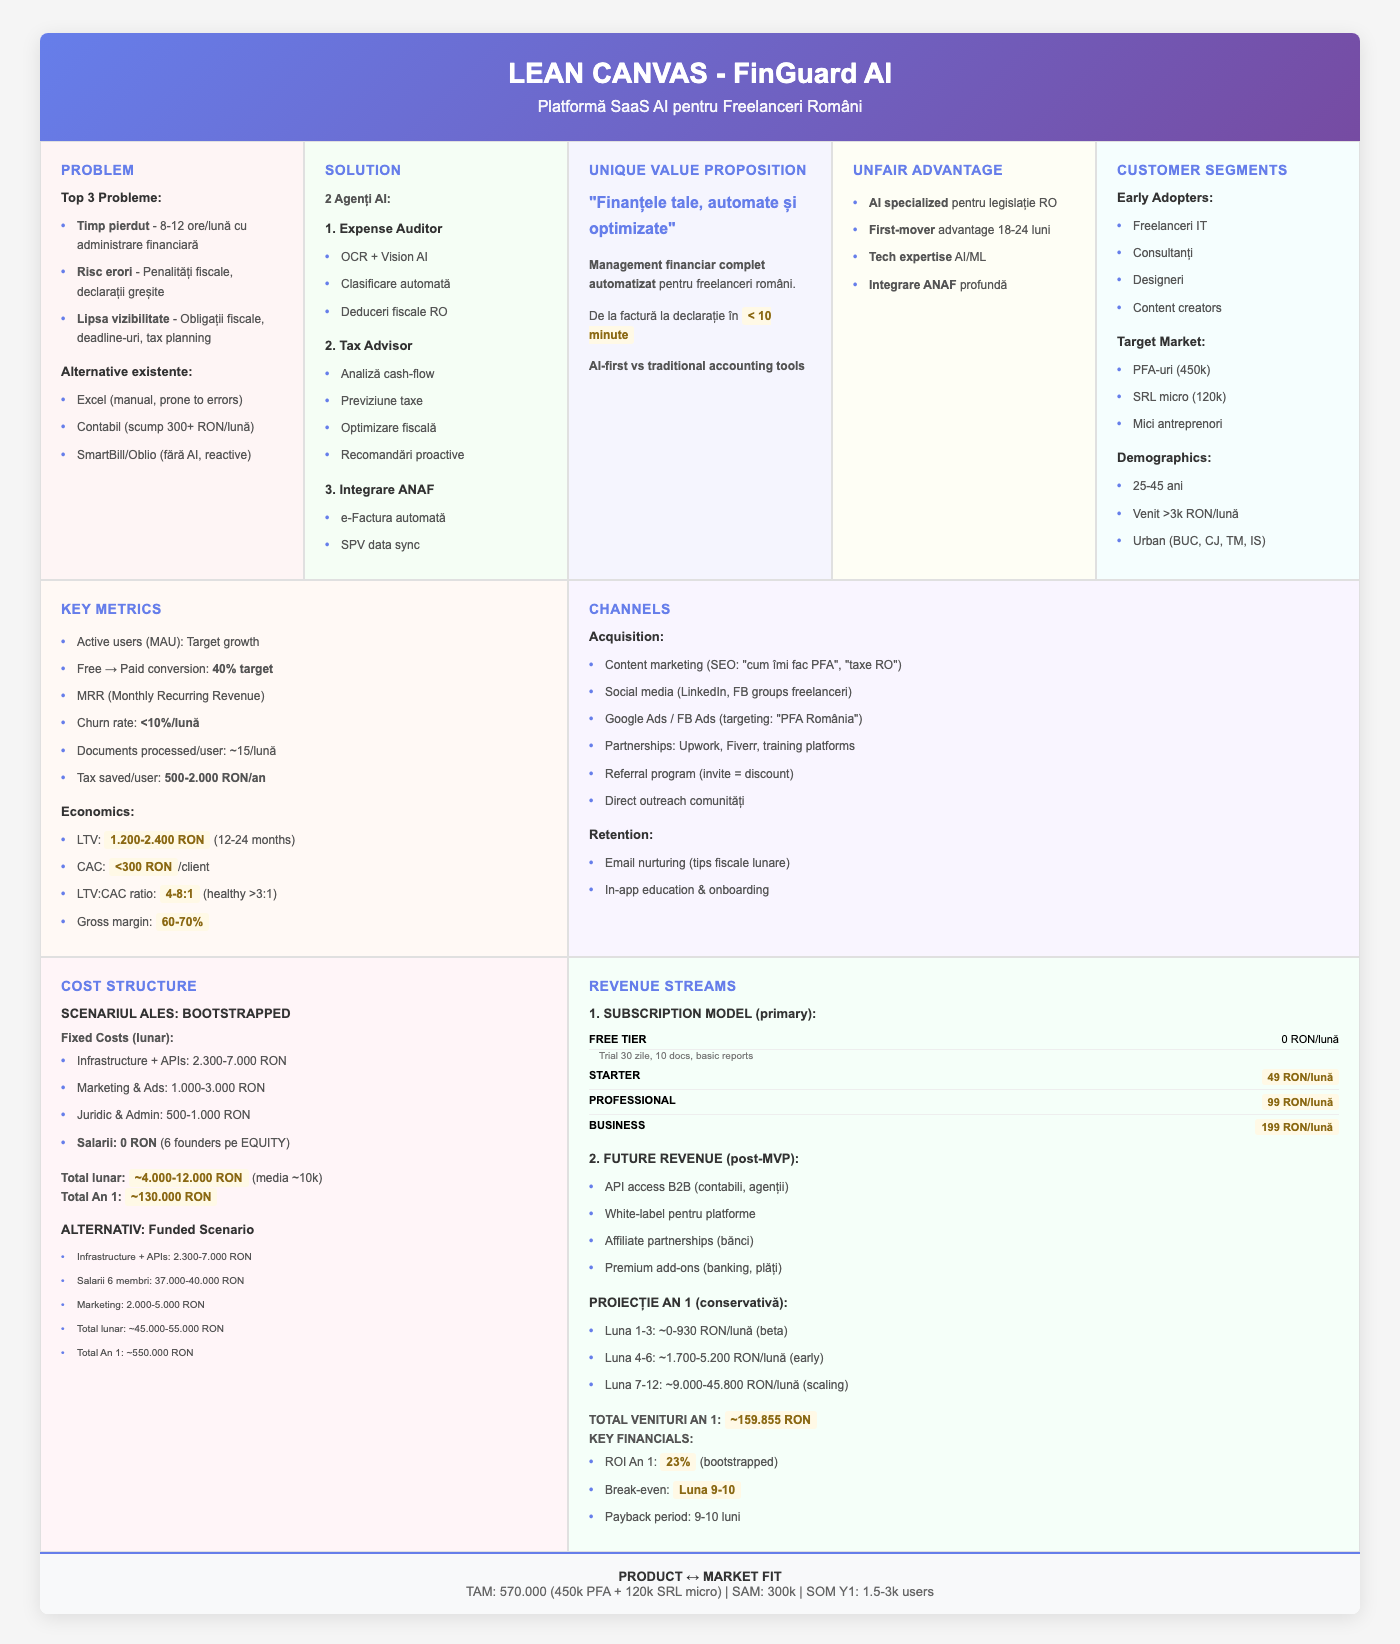
\includegraphics[width=\textwidth]{./assets/diagrams/lean-canvas.png}
\caption{Lean Canvas - FinGuard AI (Model Business 1-Page Summary)}
\end{figure}

\begin{center}
\textbf{PRODUCT $\leftrightarrow$ MARKET FIT}

TAM: 570.000 (450k PFA + 120k SRL micro) | SAM: 300k | SOM Y1: 1.5-3k users
\end{center}

\section*{Bibliografie \& Resurse}

\begin{enumerate}[nosep]
    \item \textbf{Oficiul Național al Registrului Comerțului (ONRC)} - Rapoarte statistice Q1 2026
    \item \textbf{Institutul Național de Statistică (INS)} - Câștigul salarial mediu 2025-2026
    \item \textbf{Comisia Națională de Strategie și Prognoză (CNP)} - Prognoza 2025-2028
    \item \textbf{ANAF} - Legislație fiscală, Codul Fiscal 2026, e-Factura API (\url{https://www.anaf.ro})
    \item \textbf{Plane.com} - Salarizare freelanceri remote România 2025-2026
    \item \textbf{Hacking Work / Brainspotting} - "Tech Salary \& Employment Behavior 2025"
    \item \textbf{Aviza / StartupCafe} - Analize segment PFA, impact OUG 89/2025
    \item \textbf{SmartBill, Oblio, QuickBooks, FreshBooks, Wave} - Website-uri oficiale competitori
    \item \textbf{Anthropic} - Claude API Documentation și Pricing (\url{https://anthropic.com/pricing})
    \item \textbf{NestJS, Next.js, PostgreSQL} - Documentation pentru stack-ul principal al aplicației
\end{enumerate}

\vfill

\begin{center}
\rule{0.8\textwidth}{0.4pt}\\[0.3cm]
\textbf{Document finalizat:} 29 Martie 2026 | \textbf{Versiune:} 1.0\\[0.5cm]
Universitatea din București\\
Facultatea de Matematică și Informatică\\
Management de Produs și Antreprenoriat\\
2026
\end{center}

\end{document}
